\documentclass{beamer}
\usepackage{tikz, hyperref}
\usepackage{listings}
\usepackage{pgfgantt}
\usetikzlibrary{decorations.pathreplacing}

\usetheme{terminal}

\setbeamertemplate{footline}{
  \hfill%
  \usebeamercolor[fg]{page number in head/foot}%
  \usebeamerfont{page number in head/foot}%
  \setbeamertemplate{page number in head/foot}[framenumber]%
  \usebeamertemplate*{page number in head/foot}\kern1em\vskip2pt%
}

\setbeamertemplate{navigation symbols}{} % Remove navigation symbols

\newcommand{\prompt}[1]{vtrelat@home:\raisebox{0.5ex}{\texttildelow}\$ #1}

\definecolor{cmd}{RGB}{68, 133, 96}
\definecolor{str}{RGB}{214, 175, 0}

\setcounter{framenumber}{16}
\begin{document}

\begin{frame}
    \frametitle{\prompt{echo gantt chart}}
      \begin{ganttchart}[
        hgrid,
        vgrid={*3{black,dotted}, *1{black, dashed}},
        x unit=0.32cm,
        y unit title=0.4cm,
        y unit chart=0.5cm,
        title height=1,
        title/.style={fill=gray!20},
        title label font=\bfseries\scriptsize,
        group/.append style={fill=green!20!black!70},
        bar/.style={fill=green!35!black!50},
        bar height=0.5,
        bar label font=\scriptsize,
        % progress label text={\pgfmathprintnumber[precision=0,verbatim]{#1}\%},
        group left shift=0,
        group right shift=0
      ]{1}{24}
    
      \scriptsize
      % Months every 4 units
      \gantttitle{March}{4}
      \gantttitle{April}{4}
      \gantttitle{May}{4}
      \gantttitle{June}{4}
      \gantttitle{July}{4}
      \gantttitle{August}{4}\\
      
      \ganttgroup{Porting old theories}{1}{5} \\
      \ganttbar{Reading documentation}{1}{2} \\
      \ganttbar{Fixing proofs}{2}{5} \\ \ganttnewline
      
      \ganttgroup{Time Complexity Analysis}{6}{22} \\
      \ganttbar{Paper proof}{6}{12} \\
      \ganttbar{Getting used to NREST}{9}{13} \\
      \ganttbar{Isabelle formalization}{13}{21} \\
      \ganttbar[bar/.append style={fill=orange!60}]{Proof of \texttt{estimate2\_decrease}}{14}{18} \\
      \ganttbar{Writing documentation}{19}{22}
      \end{ganttchart}
    
    \end{frame}

\begin{frame}
\frametitle{\prompt{show stats}}
\small
Beginning of the project (in SLoC):
\begin{itemize}
    \item<2-> \scriptsize{{\color{cmd}find} .\ -type f -name {\color{str}'*'} | {\color{cmd}xargs wc} -l | {\color{cmd}grep} {\color{str}'total'}}

    \small{\color{red}477020 total}
    \item<3-> \scriptsize{{\color{cmd}find} .\ -type f -name {\color{str}'*.thy'} | {\color{cmd}xargs wc} -l | {\color{cmd}grep} {\color{str}'total'}}
    
    \small{\color{red}139052 total}
\end{itemize}

Current state (in SLoC) after approx. 900h:
\begin{itemize}
    \item<4-> \scriptsize{{\color{cmd}find} .\ -type f -name {\color{str}'*'} | {\color{cmd}xargs wc} -l | {\color{cmd}grep} {\color{str}'total'}}
    
    \small{\color{red}691703 total}
    \item<5-> \scriptsize{{\color{cmd}find} .\ -type f -name {\color{str}'*.thy'} | {\color{cmd}xargs wc} -l | {\color{cmd}grep} {\color{str}'total'}}
    
    \small{\color{red}273752 total}
\end{itemize}

\onslide<6->{
\begin{center}
    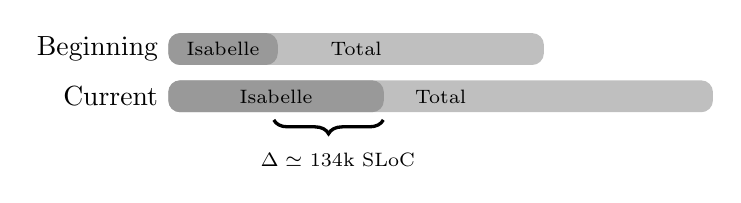
\begin{tikzpicture}[nodes={draw=none, anchor=west, minimum height=0.4cm, rounded corners=.15cm}]
        \node[fill=gray!50,   minimum width=4.77020cm] (total1) at (0,0) {\scriptsize Total};
        \node[fill=gray!80, minimum width=1.39052cm] (isa1) at (0,0) {\scriptsize Isabelle};
        \node[anchor=east] (total1lbl) at (0, 0) {Beginning};
        \node[fill=gray!50,   minimum width=6.91703cm] (total2) at (0,-.6cm) {\scriptsize Total};
        \node[fill=gray!80, minimum width=2.73752cm] (isa2) at (0,-.6cm) {\scriptsize Isabelle};
        \node[anchor=east] (total1lbl) at (0, -.6cm) {Current};

        \draw [very thick, decorate,decoration={brace,amplitude=5pt,mirror,raise=.2cm}] (1.34702cm,-.7cm) -- (2.73752cm,-.7cm) node[midway,xshift=-1cm, yshift=-.7cm]{\scriptsize$\Delta \simeq$ 134k SLoC};
    \end{tikzpicture}
\end{center}
}
\end{frame}

\end{document}
